\chapter{Resultados} \label{cap:resultados}

Nessa sessão, os resultados serão dados em termos da área medida entre a diferença da \ac{PDF} real e a estimada, como previamente mencionado. Nas figuras que seguem , os valores serão mostrados no eixo vertical, nomeado de \textit{Erro}. O eixo horizontal mostra quatro perspectivas diferentes: Probabilidade, Eixo $ x $ (que seria os valores aleatórios da variável), Primeira derivada, e segunda derivada. Essas perspectivas diferentes irão permitir um melhor entendimento das características de cada método. Cada gráfico será completado com 100 pontos de dados, cada um representando o erro medido encontrado em cada \ac{RoI} (Contudo, nessa sessão, serão considerados 100 \ac{RoI} ao invés de 20 como mostrado na Figura~\ref{fig:error}). Essa sessão será será dividida em três análises diferentes. Sessão~\ref{cap:interp_neares} analisa a estimação de erro quando a interpolação pelo vizinho mais próximo é usada; Sessão~\ref{cap:interp_lin} avalia para a interpolação linear; e a Sessão~\ref{cap:interp_neares} insere problemas de \textit{outliers}. Quando \textit{outliers} são gerados, o desempenho de alguns métodos de discretização podem ser altamente degradados em comparação com outros, sendo uma questão importante a ser analisada.

\section{Estimação de erro pela interpolação do vizinho mais próximo} \label{cap:interp_neares}
A interpolação pelo vizinho mais próximo basicamente atribui o valor vizinho mais próximo ao valor da probabilidade da variável aleatória que será estimada. Portanto, o erro de estimação será proporcional à sua distância da amostra mais próxima. Tal método de interpolação produz um erro diretamente proporcional à primeira derivada \cite{gurevich1966integral}. Analisando as Figura~\ref{fig:12a} e \ref{fig:12b} pode-se inferir que: 

\begin{figure}[H]
	\centering
	\begin{subfigure}[b]{0.45\textwidth}
		\centering 
		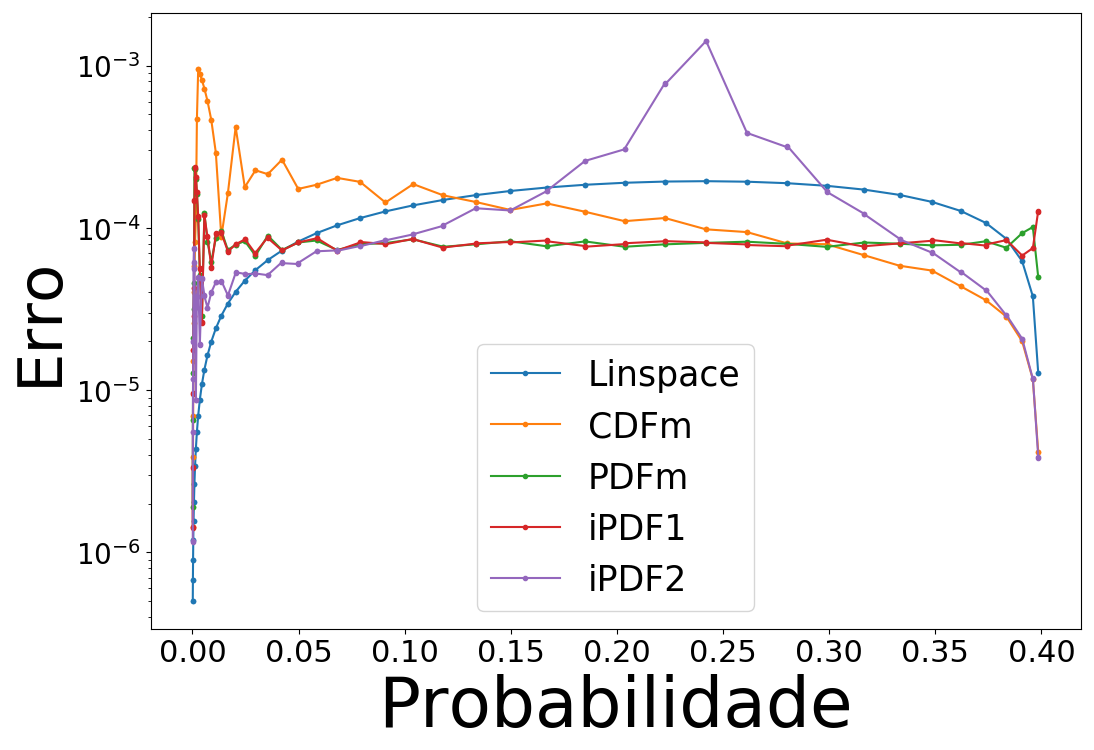
\includegraphics[width=\textwidth]{./figuras/error_normal_nearest_Probabilidade}
		\caption{}
		\label{fig:12a}
	\end{subfigure}
	\hfill
	~ %add desired spacing between images, e. g. ~, \quad, \qquad, \hfill etc. 
	%(or a blank line to force the subfigure onto a new line)
	\begin{subfigure}[b]{0.45\textwidth}
		\centering 
		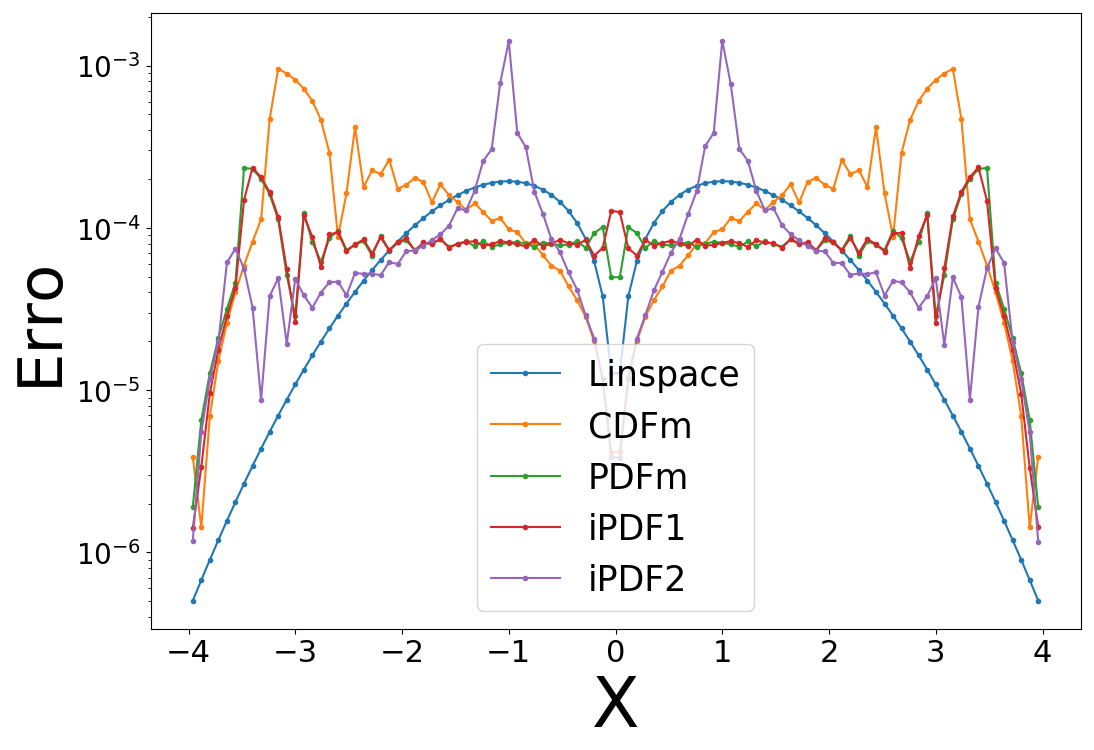
\includegraphics[width=\textwidth]{./figuras/error_normal_nearest_X}
		\caption{}
		\label{fig:12b}
	\end{subfigure}
	%\vskip\baselineskip
	~ %add desired spacing between images, e. g. ~, \quad, \qquad, \hfill etc. 
	%(or a blank line to force the subfigure onto a new line)
	\begin{subfigure}[b]{0.45\textwidth}
		\centering 
		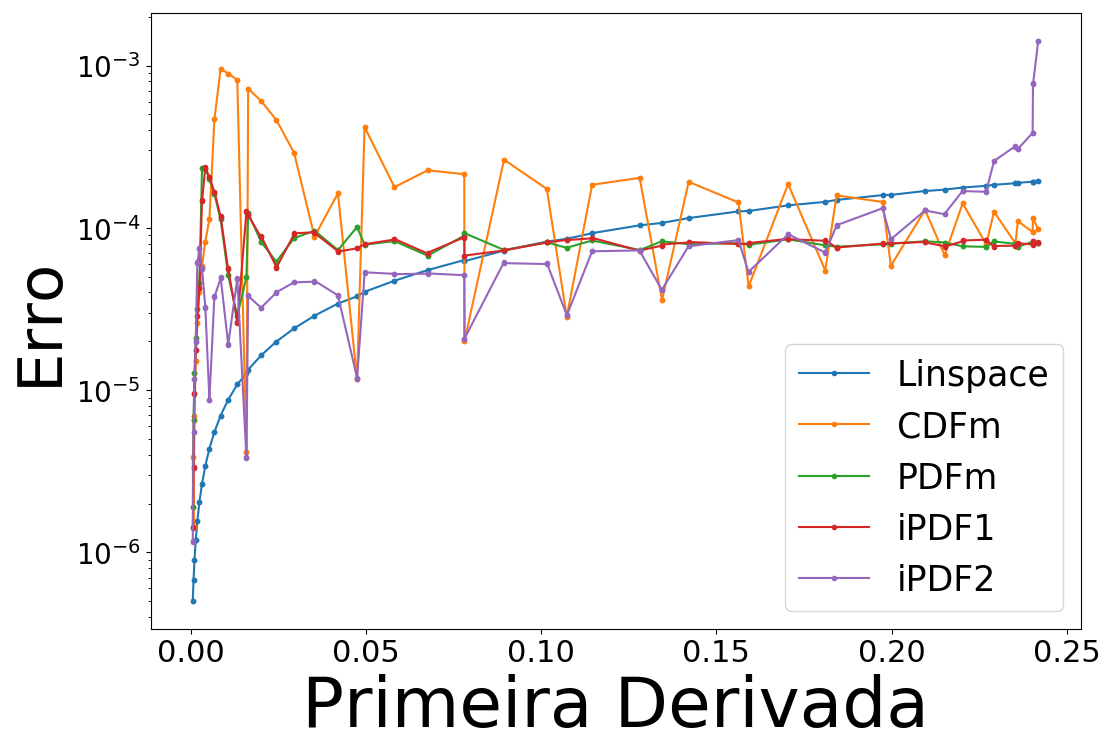
\includegraphics[width=\textwidth]{./figuras/error_normal_nearest_Primeira_Derivada.png}
		\caption{}
		\label{fig:12c}
	\end{subfigure}
	\hfill
	\begin{subfigure}[b]{0.45\textwidth}
		\centering 
		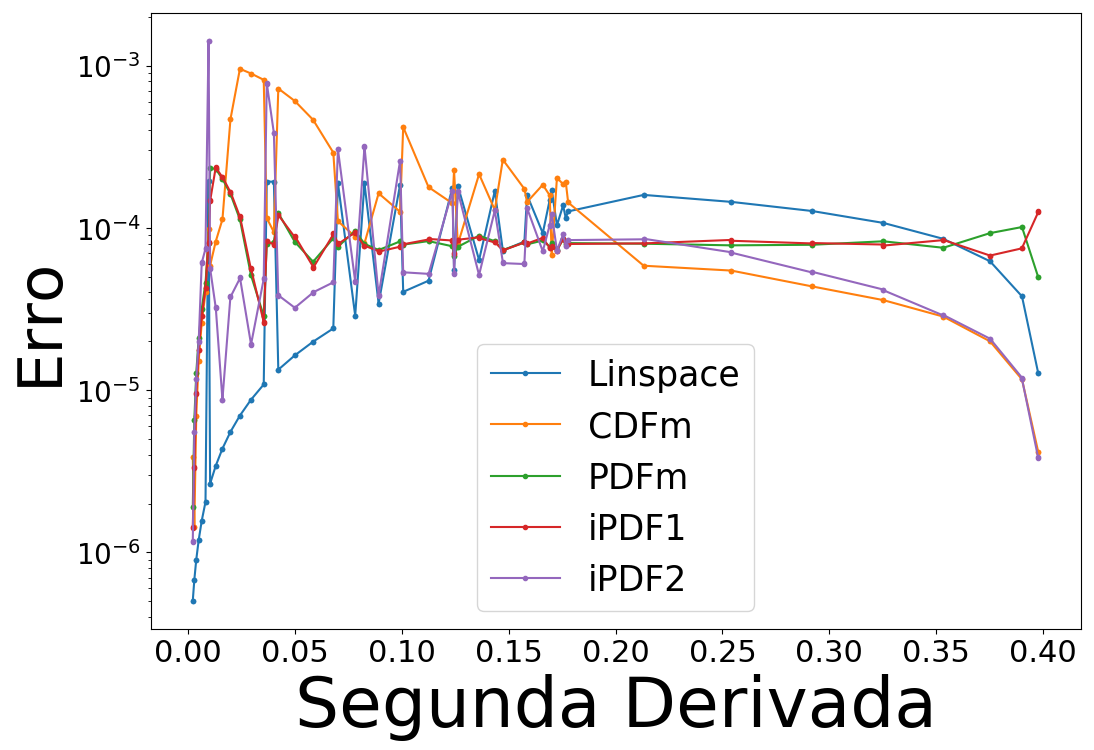
\includegraphics[width=\textwidth]{./figuras/error_normal_nearest_Segunda_Derivada.png}
		\caption{}
		\label{fig:12d}
	\end{subfigure}
	\caption{Caso representativo com 200 pontos, 100 \ac{RoI} e usando a interpolação pelo vizinho mais próximo.}
	\label{fig:12}
\end{figure}

\begin{description}
	\item[Linspace] erro de estimação aumenta com a 1ª derivada da função que está sendo estimada;
	\item[CDFm] erro de estimativa diminui com o aumento da probabilidade; 
	\item[PDFm e iPDF1] tendem a equalizar o erro de estimativa aumentando a densidade de pontos discretos nas regiões de derivadas mais altas; 
	\item[iPDF2] diminui o erro com o aumento da probabilidade, no entanto, apresenta um aumento de erro próximo ao ponto de inflexão.
\end{description}  

Na Figura~\ref{fig:12c} é possível perceber que:
 \begin{description}
	\item[Linspace] apresenta um aumento do erro de estimação diretamente proporcional ao valor da 1ª derivada;
	\item[CDFm] apresenta maior densidade de pontos na região de alta probabilidade e poucos pontos na região de baixa probabilidade. No entanto, do ponto de vista da 1ª derivada, o erro de estimação oscila entre valores altos e baixos;
	\item[PDFm e iPDF1] tendem a manter constante o valor do erro de estimação, uma vez que se coloca mais pontos em regiões com derivadas maiores, onde o erro do método de discretização pelo vizinho mais próximo é maior. Porém, como mencionado anteriormente, as caudas apresentam os menores erros, o que justifica a diminuição do erro nas regiões de baixa derivada;
	\item[iPDF2] aumenta o erro de estimação de acordo com o aumento da 1ª derivada, uma vez que tais regiões tendem a receber menos pontos estimados.
\end{description}  

Finalmente, quando a Figura \ref{fig:12d} é observada (lembrando que valores baixos de 2ª derivada representam regiões intercaladas de baixa probabilidade e inflexão, de modo que, estas são as situações onde o erro causado pela interpolação é menor) ela pode ser inferida que:

\begin{description}
	\item[Linspace e iPDF2] exibem comportamento similar, aumentam o erro diretamente proporcional à 2ª derivada, porém, ao se aproximarem da região de alta probabilidade, o erro tende a cair;
	\item[CDFm] tende a diminuir em erro a medida que a segunda derivada aumenta;
	\item[PDFm e iPDF1] não parecem sofrer com a variação da 2ª derivada, exceto em regiões de valores baixos, onde o erro flutua.
\end{description}

Podemos também realizar uma análise de desempenho verificando a equivalência do erro de estimação para quando o número estimado varia, conforme mostra a Figura~\ref{fig:errorplotnearest}.

\begin{figure}[H]
	\centering
	\begin{subfigure}[b]{0.45\textwidth}
		\centering 
		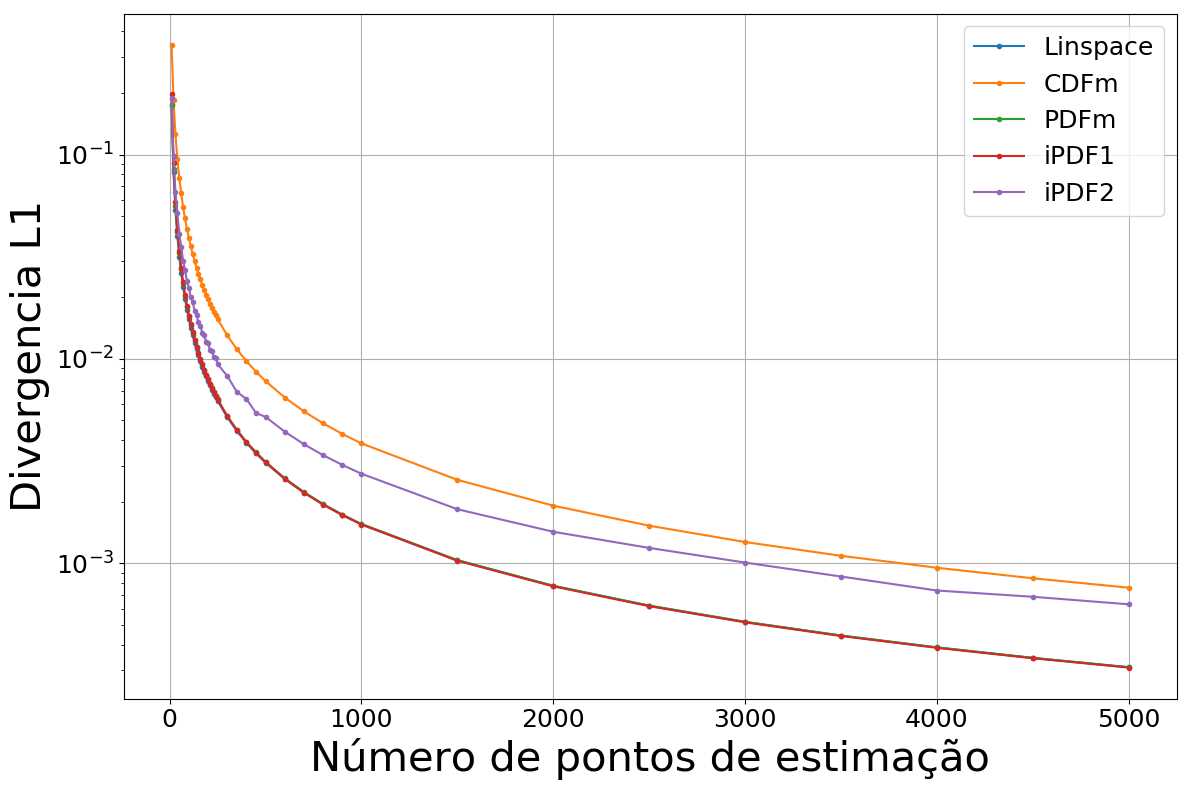
\includegraphics[width=\textwidth]{./figuras/ERRORPLOT_L1_TRUE_NORMAL_NEAREST_00}
		\caption{}
		\label{fig:errornormnearest}
	\end{subfigure}
	\hfill
	~ %add desired spacing between images, e. g. ~, \quad, \qquad, \hfill etc. 
	%(or a blank line to force the subfigure onto a new line)
	\begin{subfigure}[b]{0.45\textwidth}
		\centering 
		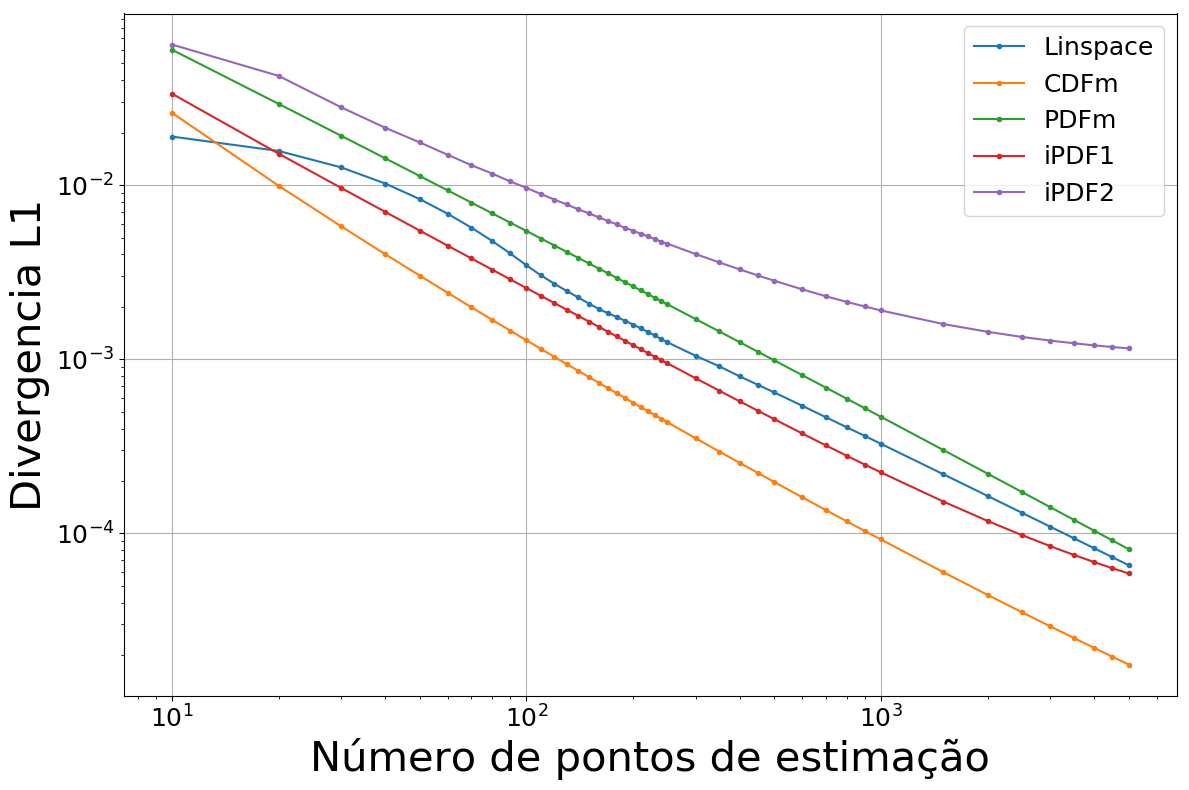
\includegraphics[width=\textwidth]{./figuras/ERRORPLOT_L1_TRUE_LOGNORMAL_NEAREST_00}
		\caption{}
		\label{fig:errorlognearest}
	\end{subfigure}
	
	\caption{Erro total de estimação para a interpolação pelo vizinho mais próximo variando-se o números de pontos a se estimar: (a) N(0,1) e (b) L(0,1)}
	\label{fig:errorplotnearest}
\end{figure}

Podemos perceber que na Figura~\ref{fig:errornormnearest}, devido ao fato de possuir uma derivada mais lenta, o método \textit{Linspace} é o que possui o menor erro, juntamente com os métodos \ac{PDFm} e \ac{iPDF1}, por outro lado, o método \ac{CDFm} é o que possui o pior desempenho, fazendo com que se necessite de mais pontos de estimação para possuir o mesmo erro total que os outros métodos. Já quando a distribuição possui uma variação maior, a cena se inverte, como é mostrada na Figura~\ref{fig:errorlognearest} em que a \ac{CDFm} é a que possui o menor erro, sendo necessário, por exemplo possuir apenas 120 pontos de estimação enquanto o \textit{Linspace} necessita de 300 pontos para manter o mesmo erro.


\section{Estimação de erro pela interpolação linear} \label{cap:interp_lin}

O método de interpolação linear naturalmente tende a apresentar erros de estimação mais altos em regiões com a 2ª derivada maior se os pontos discretos forem distribuídos uniformemente ao longo do eixo horizontal, como pode ser notado pelo método \textit{Linspace} da Figura \ref{fig:11d}. Adicionalmente, analisando as Figuras \ref{fig:11a} e \ref{fig:11b} é possível observar o seguinte:

\begin{description}
	\item[Linspace] erro de estimação diminui em regiões de baixa probabilidade e perto dos pontos de inflexão;
	\item[CDFm] erro de estimação diminui com o aumento da probabilidade, e nos pontos de inflexão há uma melhoria ainda maior;
	\item [PDFm e iPDF1] erro aumenta em regiões de baixa e alta probabilidade e diminui próximo aos pontos de inflexão;
	\item[iPDF2] apresenta menor densidade de pontos em regiões de baixa probabilidade e regiões de inflexão, levando a um comportamento inverso quando comparado ao método \textit{Linspace}.
\end{description}   

\begin{figure}[H]
	\centering
	\begin{subfigure}[b]{0.45\textwidth}
		\centering 
		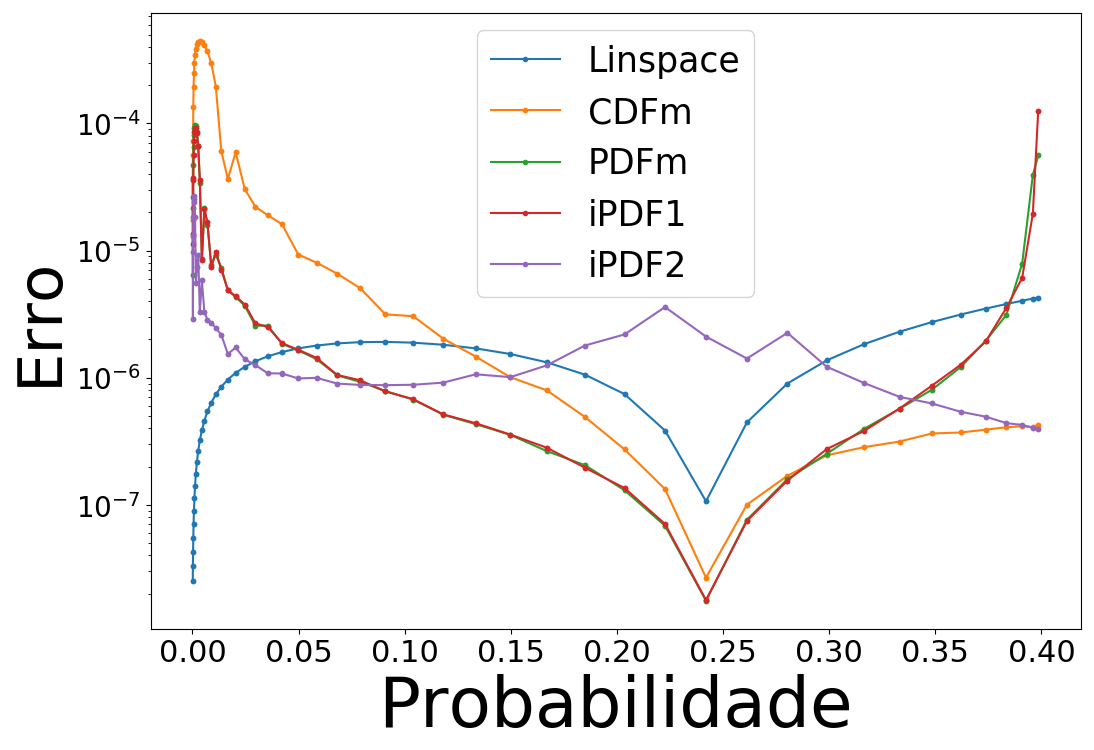
\includegraphics[width=\textwidth]{./figuras/error_normal_linear_Probabilidade}
		\caption{}
		\label{fig:11a}
	\end{subfigure}
	\hfill
	~ %add desired spacing between images, e. g. ~, \quad, \qquad, \hfill etc. 
	%(or a blank line to force the subfigure onto a new line)
	\begin{subfigure}[b]{0.45\textwidth}
		\centering 
		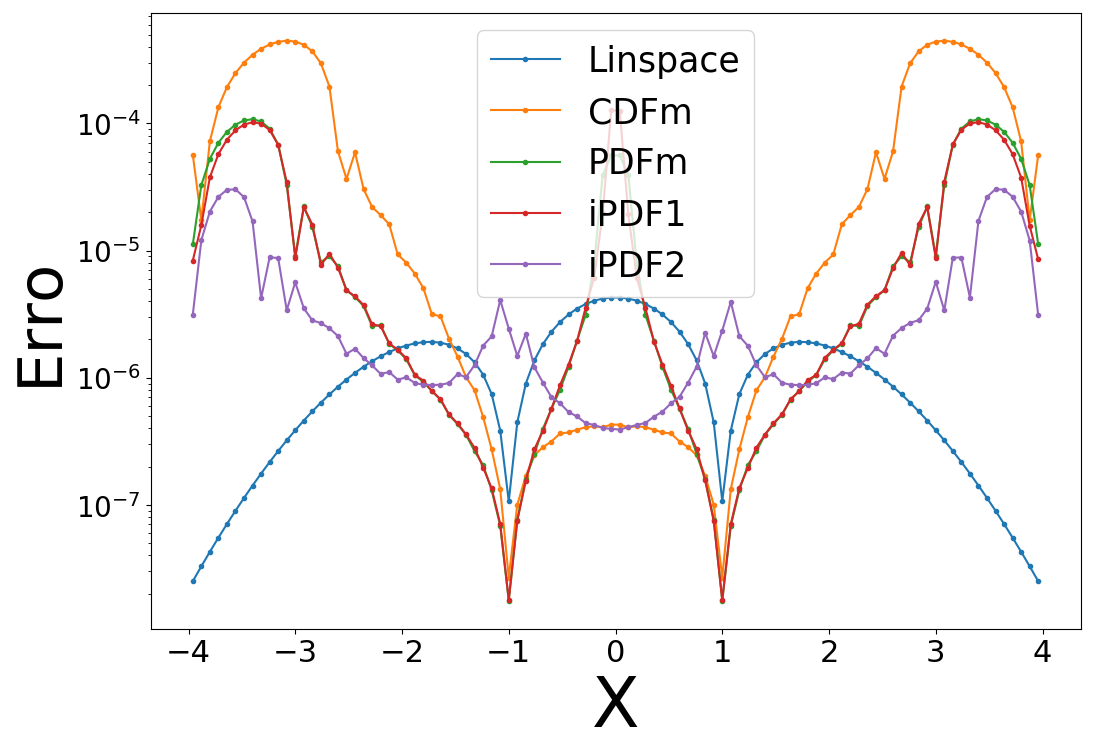
\includegraphics[width=\textwidth]{./figuras/error_normal_linear_X}
		\caption{}
		\label{fig:11b}
	\end{subfigure}
	%\vskip\baselineskip
	~ %add desired spacing between images, e. g. ~, \quad, \qquad, \hfill etc. 
	%(or a blank line to force the subfigure onto a new line)
	\begin{subfigure}[b]{0.45\textwidth}
		\centering 
		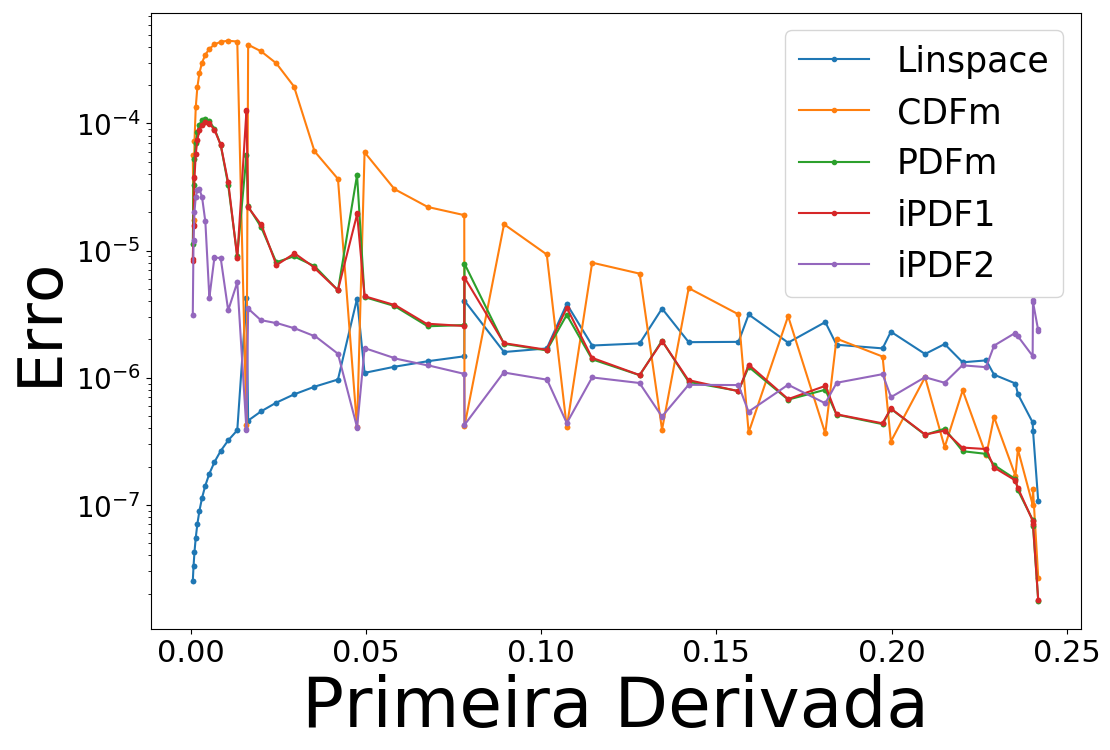
\includegraphics[width=\textwidth]{./figuras/error_normal_linear_Primeira_Derivada.png}
		\caption{}
		\label{fig:11c}
	\end{subfigure}
	\hfill
	\begin{subfigure}[b]{0.45\textwidth}
		\centering 
		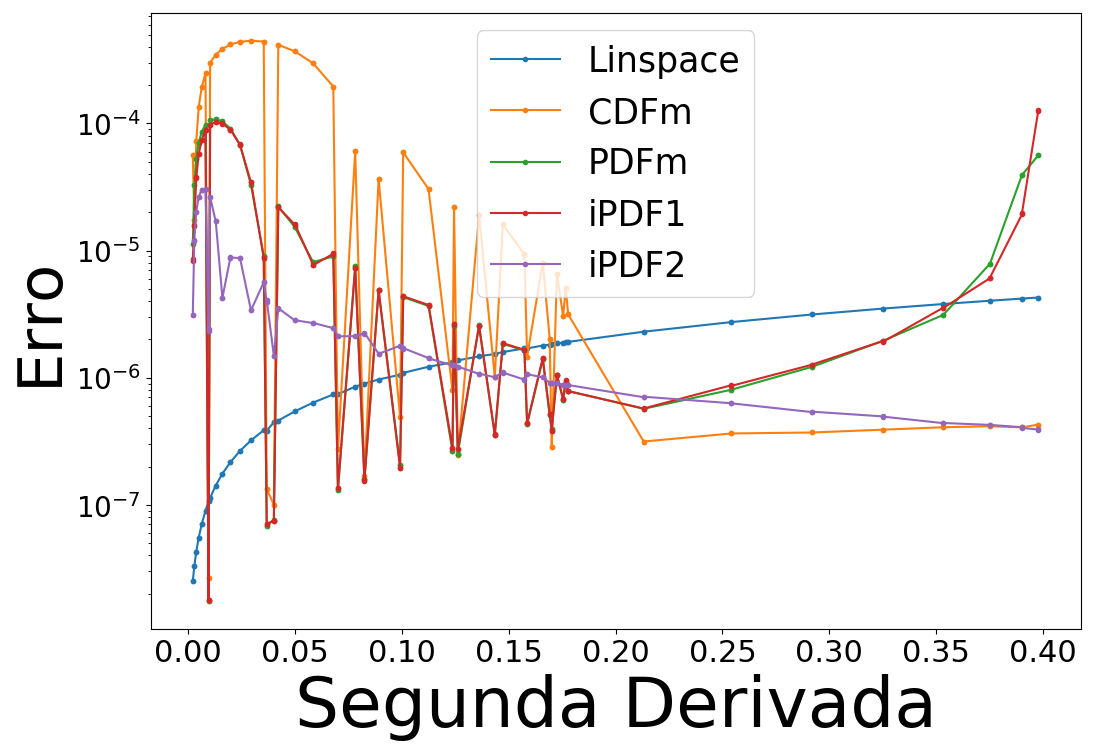
\includegraphics[width=\textwidth]{./figuras/error_normal_linear_Segunda_Derivada.png}
		\caption{}
		\label{fig:11d}
	\end{subfigure}
	
	\caption{Caso representativo com 200 pontos, 100 \ac{RoI} e usando a interpolação linear.}\label{fig:11}
\end{figure}

Avaliando a Figura \ref{fig:11c} é possível confirmar que os métodos \textit{Linspace} e \ac{iPDF2} têm comportamentos opostos. Os outros métodos se comportam de maneira semelhante, pois reduzem o erro de estimação quando a 1ª derivada aumenta.
Na Figura \ref{fig:11d}, é possível notar que o método \textit{Linspace} mostra a mesma tendência em relação à 2ª derivada para o caso da interpolação linear da apresentada em relação à 1ª derivada para o caso da interpolação pelo vizinho mais próximo.
A flutuação de erro observada no método \ac{CDFm} é causada pela variação entre as regiões de alta e baixa probabilidade ao longo do eixo da 2ª derivada, no entanto, uma vez que as regiões de alta probabilidade estão associadas à regiões de segunda derivada alta, esta oscilação tende a desaparecer com o aumento desta derivada.
Isso também explica as flutuações nos métodos \ac{PDFm} e \ac{iPDF1}, porém esses métodos apresentam desempenho degradado em regiões de alta probabilidade. Finalmente, o método \ac{iPDF2} mantém o comportamento inverso ao método \textit{Linspace}.

Ao mudarmos para a interpolação linear, é possível perceber que o erro diminui de maneira considerável, como pode ser visto na Figura~\ref{fig:errorplotlin} em que para a distribuição Normal, o método \textit{Linspace} se sobressai a todos os outros e, como na interpolação pelo vizinho mais próximo o método \ac{CDFm} é o pior, como ilustra a Figura~\ref{fig:errornormlin}, já para a distribuição Lognormal, o método \ac{CDFm} se sobressai até os 1000 pontos de estimação, após o método \textit{Linspace} se torna mais eficiente como é ilustrado na Figura~\ref{fig:errorloglin} devido ao fato de ser o único método que estima com maior precisão as regiões de baixa probabilidade.

\begin{figure}[H]
	\centering
	\begin{subfigure}[b]{0.45\textwidth}
		\centering 
		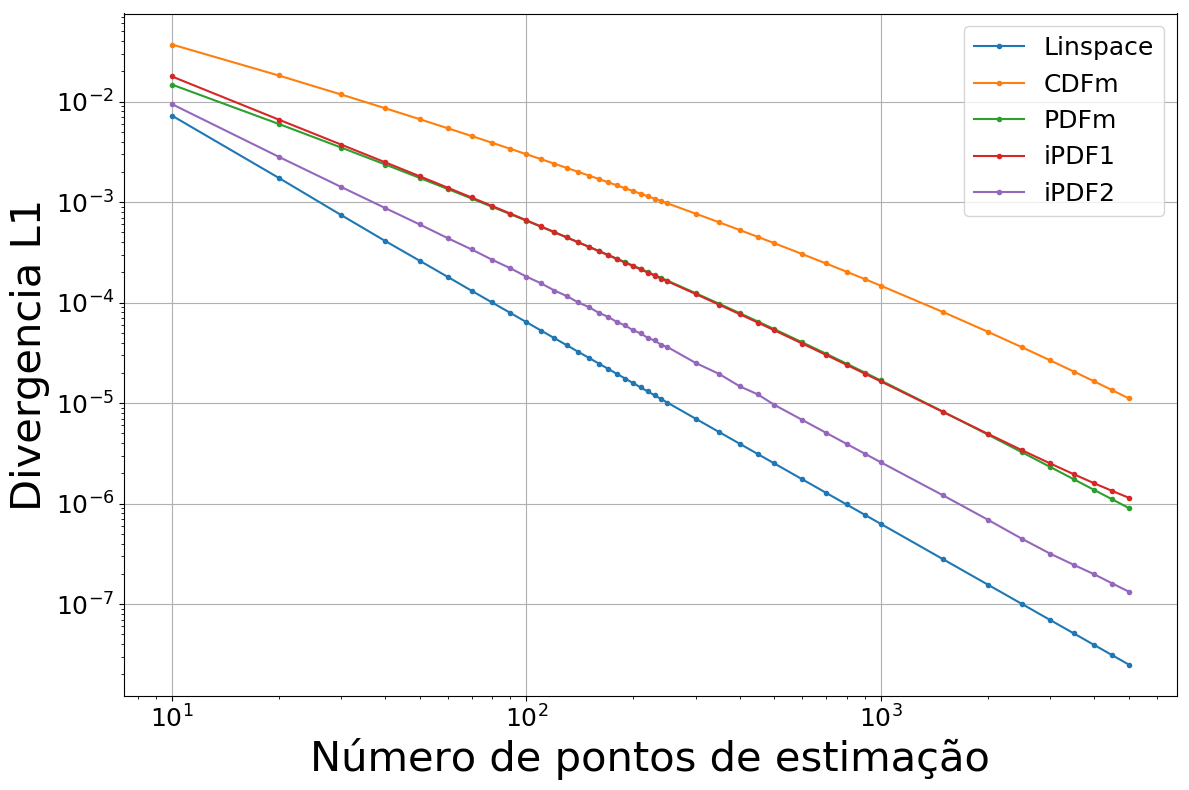
\includegraphics[width=\textwidth]{./figuras/ERRORPLOT_L1_TRUE_NORMAL_LINEAR_00}
		\caption{}
		\label{fig:errornormlin}
	\end{subfigure}
	\hfill
	~ %add desired spacing between images, e. g. ~, \quad, \qquad, \hfill etc. 
	%(or a blank line to force the subfigure onto a new line)
	\begin{subfigure}[b]{0.45\textwidth}
		\centering 
		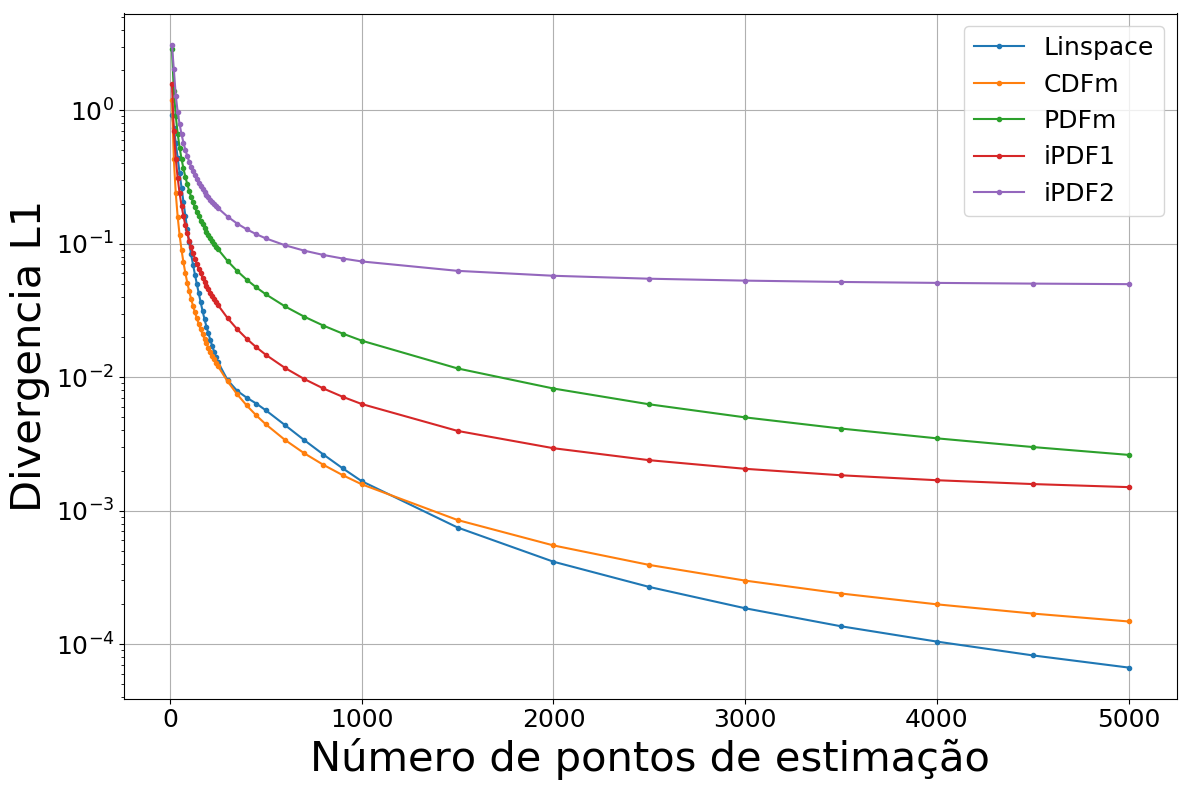
\includegraphics[width=\textwidth]{./figuras/ERRORPLOT_L1_TRUE_LOGNORMAL_LINEAR_00}
		\caption{}
		\label{fig:errorloglin}
	\end{subfigure}
	
	\caption{Erro total de estimação para a interpolação linear variando-se o números de pontos a se estimar: (a) N(0,1) e (b) L(0,1)}
	\label{fig:errorplotlin}
\end{figure}

\section{Estimação de erro considerando \textit{outliers}} \label{cap:erro_out}

A fim de verificar o comportamento dos métodos de discretização em uma realidade onde existem conjuntos de dados com \textit{outliers}, como é comum em experimentos reais, \textit{outliers} foram inseridos nos dados gerados. As posições \textit{outliers} foram varridas até o valor de 50.
O problema dos \textit{outliers} pode ser visto de outra perspectiva, relacionado à definição dos limites do eixo horizontal, que é geralmente um pré-requisito para aplicar algoritmos de estimativa de \ac{PDF}.
Além disso, o número de pontos estimados foi varrido para 1000. Esta análise pode ser vista na Figura~\ref{fig:13}.

\begin{figure}[H]
	\centering
	\begin{subfigure}[b]{0.45\textwidth}
		\centering 
		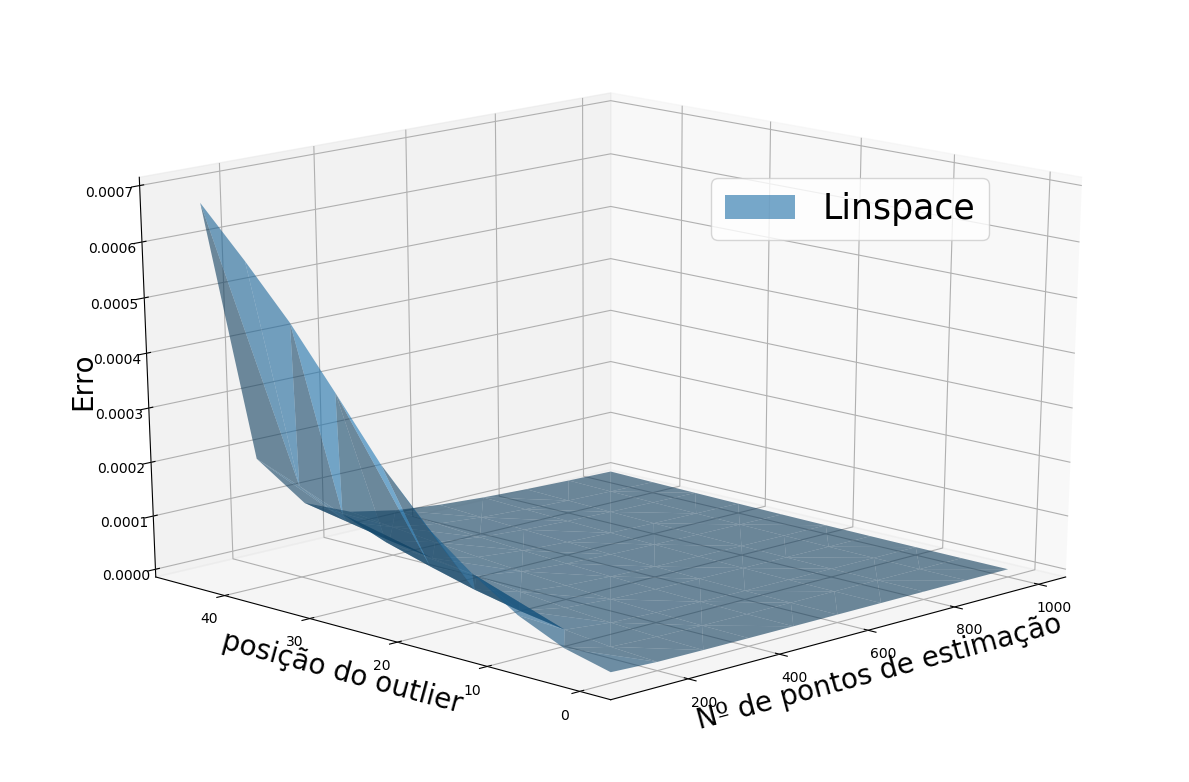
\includegraphics[width=\textwidth]{./figuras/erro3d_linspace}
		\caption{}
		\label{fig:13a}
	\end{subfigure}
	\hfill
	\begin{subfigure}[b]{0.45\textwidth}
		\centering 
		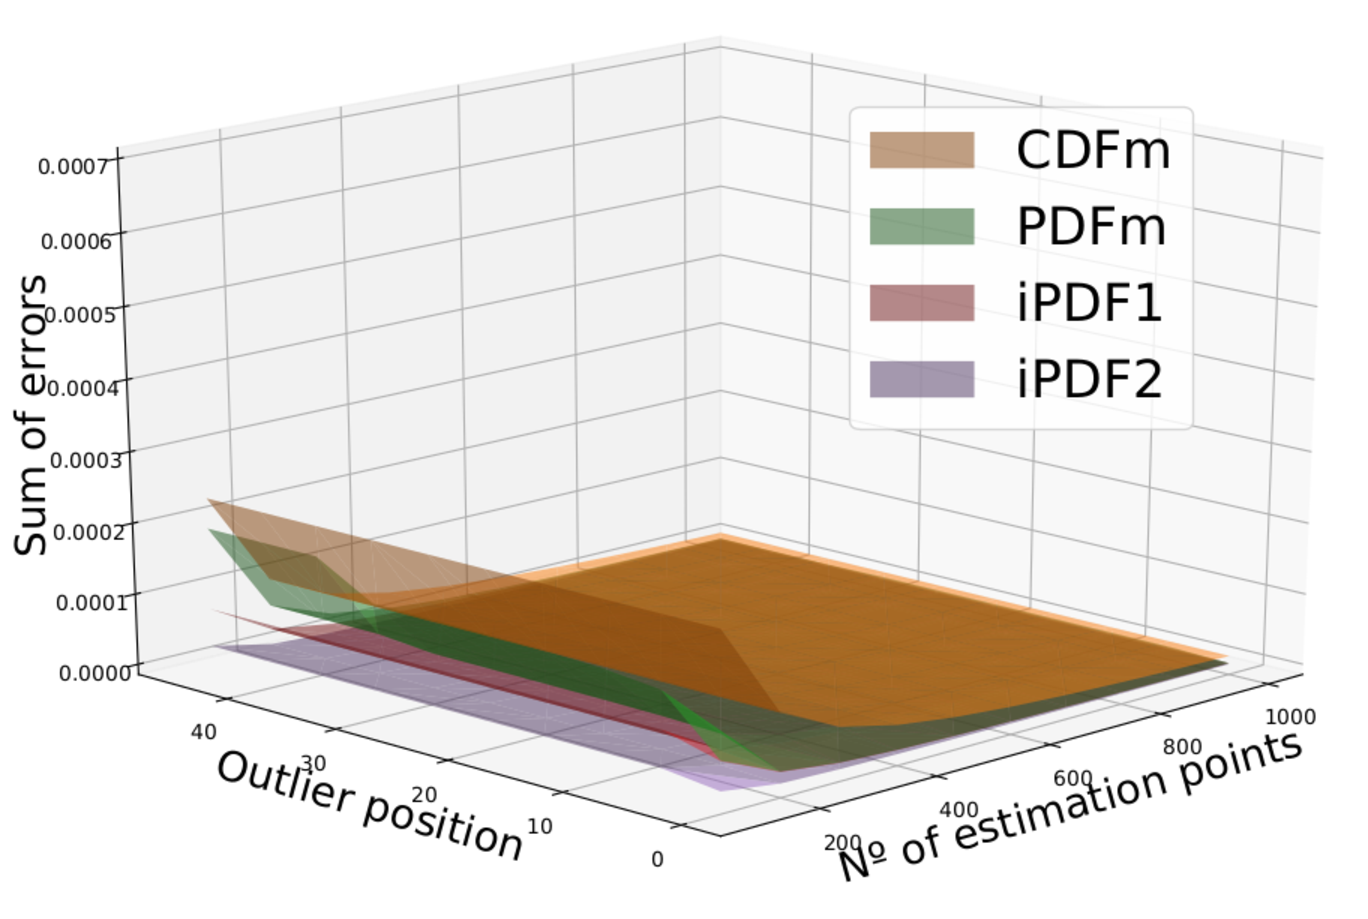
\includegraphics[width=\textwidth]{./figuras/figure13b.pdf}
		\caption{}
		\label{fig:13b}
	\end{subfigure}
	\caption{Análise de \textit{outlier} usando 100 Rois e interpolação linear.}
	\label{fig:13}
\end{figure}

A figura \ref{fig:13a} mostra que o método \textit{Linspace} aumenta consideravelmente seu erro de estimação quando \textit{outliers} são inseridos; quanto mais distantes os \textit{outliers}, maior o erro. Este efeito é mitigado pelo aumento do número de pontos estimados.
A Figura~\ref{fig:13b} mostra que os métodos propostos são menos sensíveis aos \textit{outliers} (ou à escolha dos limites do eixo horizontal). As tabelas \ref{tab:near} e \ref{tab:lin} mostram o erro médio dos métodos para três posições de \textit{outliers} (0, 20 e 50) e 100 pontos de estimação), para interpolações do vizinho mais próximo e linear, respectivamente.

\begin{table}[H]
	\centering
	\caption{Erro de estimativa média usando a distribuição normal e interpolação do vizinho mais próximo com 100 pontos de estimação.}
	\label{tab:near}
	\begin{tabular}{llllll}
		\hline
		\multicolumn{6}{c}{\textbf{Média}}                                                                                             \\ \hline
		\multicolumn{1}{l|}{\textbf{\#Outlier}} & \textbf{Linspace} & \textbf{CDFm} & \textbf{PDFm} & \textbf{iPDF1} & \textbf{iPDF2} \\ \hline
		\multicolumn{1}{l|}{\textbf{0}}         & 8.02e-5           & 1.96e-4       & 8.26e-5       & 8.19e-5        & 1.20e-4        \\
		\multicolumn{1}{l|}{\textbf{20}}        & 4.82e-4           & 1.96e-4       & 1.14e-4       & 9.22e-5        & 1.25e-4        \\
		\multicolumn{1}{l|}{\textbf{50}}        & 1.09e-3           & 1.96e-4       & 1.14e-4       & 9.22e-5        & 1.25e-4        \\ \hline
	\end{tabular}
	
\end{table}

\begin{table}[H]
	\centering
	\caption{Erro de estimação média usando a distribuição normal e interpolação linear com 100 pontos de estimação.}
	\label{tab:lin}
	\begin{tabular}{llllll}
		\hline
		\multicolumn{6}{c}{\textbf{Média}}                                                                                             \\ \hline
		\multicolumn{1}{l|}{\textbf{\#Outlier}} & \textbf{Linspace} & \textbf{CDFm} & \textbf{PDFm} & \textbf{iPDF1} & \textbf{iPDF2} \\ \hline
		\multicolumn{1}{l|}{\textbf{0}}         & 1.30e-6           & 1.01e-4       & 2.14e-5       & 2.07e-5        & 4.97e-6        \\
		\multicolumn{1}{l|}{\textbf{20}}        & 4.66e-5           & 1.01e-4       & 5.61e-5       & 3.01e-5        & 8.35e-6        \\
		\multicolumn{1}{l|}{\textbf{50}}        & 2.31e-4           & 1.01e-4       & 6.38e-5       & 3.00e-5        & 8.35e-6      \\
		\hline
	\end{tabular}
	\
\end{table}

Para a interpolação do vizinho mais próximo, o método \ac{iPDF1} apresentou o melhor desempenho enquanto para a interpolação Linear, o \ac{iPDF2} foi o melhor se o erro de estimação e a sensibilidade de \textit{outliers} forem considerados. O \ac{CDFm} mostrou-se praticamente imune a \textit{outliers}. Quando nenhum valor discrepante está presente, o Linspace atinge o melhor resultado seguido de perto pelo \ac{PDFm} e \ac{iPDF1} para o caso do vizinho mais próximo e pelo \ac{iPDF2} para o caso Linear. No entanto, é influenciado pela escolha arbitrária de 99.99\% da área como limites do eixo horizontal padrão para caracterizar a ausência de \textit{outliers}. 
A figura~\ref{fig:Error_out} mostra como o erro varia conforme é aumentado a quantidade de pontos de estimação, sendo que, como é mostrado na Figura~\ref{fig:error_norm_near_50}, há uma mudança na performance de cada método, fazendo com que alguns se sobressaiam sobre outros conforme é aumentado o número de pontos, para este caso, utilizando a interpolação pelo vizinho mais próximo, os métodos \ac{iPDF1} e \ac{iPDF2} foram os que tiveram o menor erro até os 5000 pontos estimados. Já para a interpolação Linear, mostrada na Figura~\ref{fig:error_norm_lin_50} os métodos \ac{iPDF1}, \ac{iPDF2} e \ac{CDFm} estagnam por volta do 500º ponto de estimação, não alterando mais tanto o valor do erro após isso, em contrapartida, o método \textit{Linspace} continua a melhorar conforme o número de pontos aumenta, chegando ser o melhor a partir do 1000º ponto. 

\begin{figure}[H]
	\centering
	\begin{subfigure}[b]{0.45\textwidth}
		\centering 
		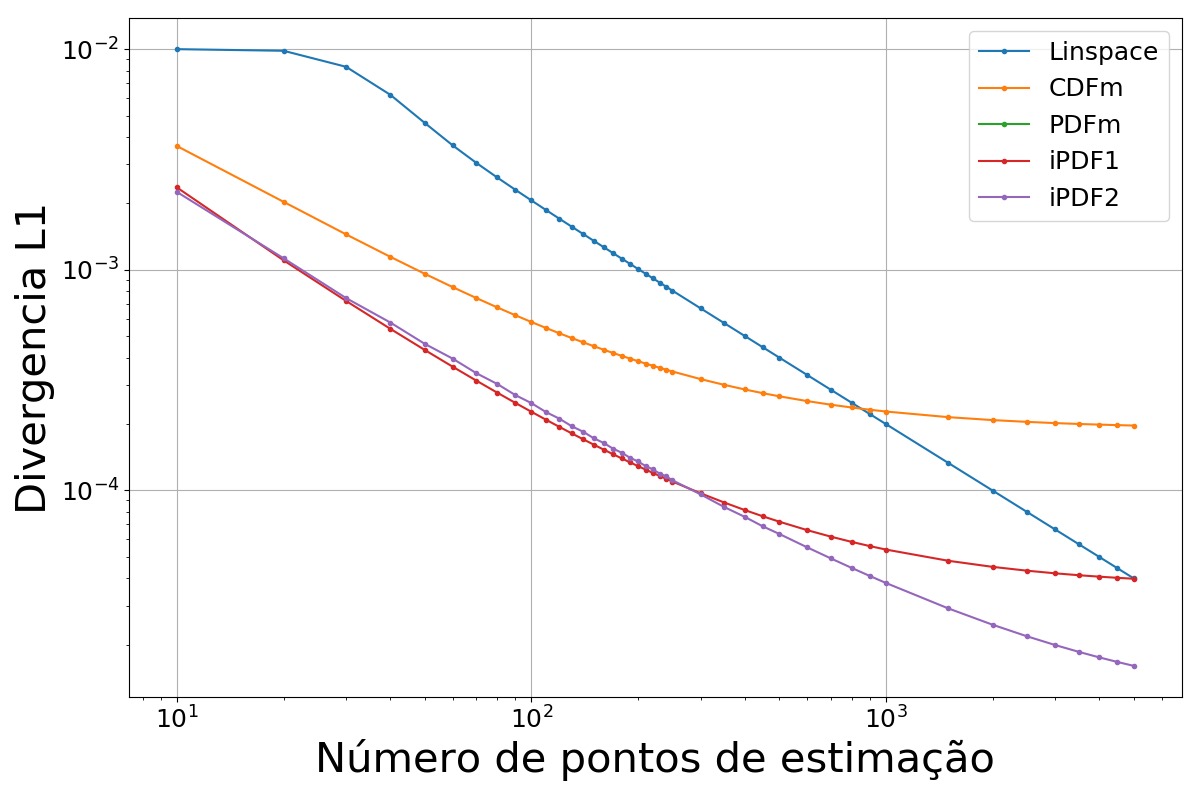
\includegraphics[width=\textwidth]{./figuras/ERRORPLOT_L1_TRUE_NORMAL_NEAREST_050_log}
		\caption{}
		\label{fig:error_norm_near_50}
	\end{subfigure}
	\hfill
	~ %add desired spacing between images, e. g. ~, \quad, \qquad, \hfill etc. 
	%(or a blank line to force the subfigure onto a new line)
	\begin{subfigure}[b]{0.45\textwidth}
		\centering 
		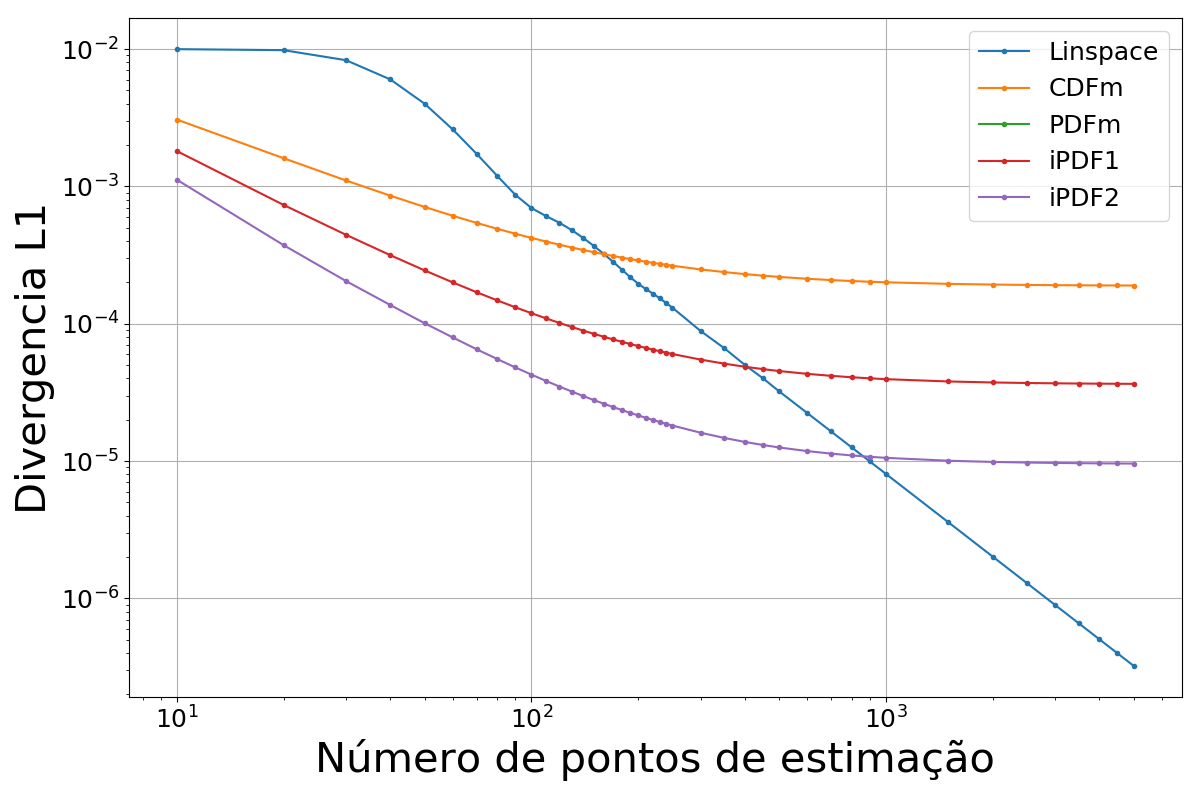
\includegraphics[width=\textwidth]{./figuras/ERRORPLOT_L1_TRUE_NORMAL_LINEAR_050_log}
		\caption{}
		\label{fig:error_norm_lin_50}
	\end{subfigure}
\caption{Erro total de estimação para a distribuição Normal com outlier em 50 (a) para a interpolação pelo vizinho mais próximo, (b) para a interpolação linear.}
\label{fig:Error_out}
\end{figure}